% Matlab Implementation of Neural Field Model
% tex file of implementation document


\documentclass[a4paper, 12pt, english]{article}


% packages
\usepackage[english]{babel}
\usepackage{setspace}
\usepackage{amsmath}
\usepackage{amsfonts}
\usepackage{bm}
\usepackage{graphicx}
\usepackage{float}
\usepackage{caption}


% graphic path
\graphicspath{{/Users/miao/Documents/Miao/Neurosciences/Projects/NeuralFieldModel/Figures/}}


% title of this manuscript
\title{Matlab Implementation of Neural Field Model}
\author{Miao Cao}
\date{1 July 2016}


\begin{document}
% set spacing of this document
\onehalfspacing

% title of the document
\begin{titlepage}\centering
\vspace*{\fill}
\maketitle
\vspace*{\fill}
\end{titlepage}

\tableofcontents

\newpage



% Introduction
\section{Introduction}
\paragraph{In order to implement and simulate Neural Field Model in Matlab, we break down
neural field model into several parts based mathematical equations and independently implement and test each part. The
following sections show the details of our implementation. Please always refer to
Freestone et al., 2011, NeuroImage for derivations, equations and details.}

\newpage



% Convolution of two Gaussians
\section{Convolution of Two Gaussian Basis Functions}

\paragraph{To test the analytic solution of convolution of two Gaussians, w
e compute the convolution of two Gaussians both analytically and numerically.
The numerical solution is to use Matlab built-in funciton conv2. By obtaining
the residual of two solutions, we are able to prove that our analytical solution
has very significantly high accuracy.}

\paragraph{File (Matlab script): Convolution2DGaussians.m}


\subsection{Implementations}
To analytically compute the convolution of two Gaussians, we use the following
equation:
$$\left(\varphi_i\ast\varphi_j\right)(\boldsymbol{r}) = \left(\frac{\pi\sigma^2_i\sigma^2_j}{\sigma^2_i + \sigma^2_j}\right)^{\frac{n}{2}}\\
\times\exp\left(-\frac{1}{\sigma^2_i + \sigma^2_j}(\boldsymbol{r}-\boldsymbol{\mu})^T(\boldsymbol{r}-\boldsymbol{\mu})\right), $$
where $\boldsymbol{\mu} = \boldsymbol{\mu_i} + \boldsymbol{\mu_j} $.
This equation is given as Equation (E.4) in Appendix E.\par

Practically, we compute the convolution of two Gaussians, $\phi$ and $\psi $,
with analytical solution (Equation E.4) and numerical solution (Matlab
buit-in function \textit{conv2}).
The residual of two solutions are presented in the next section.


\subsection{Results}
\begin{figure}[H]
\centering
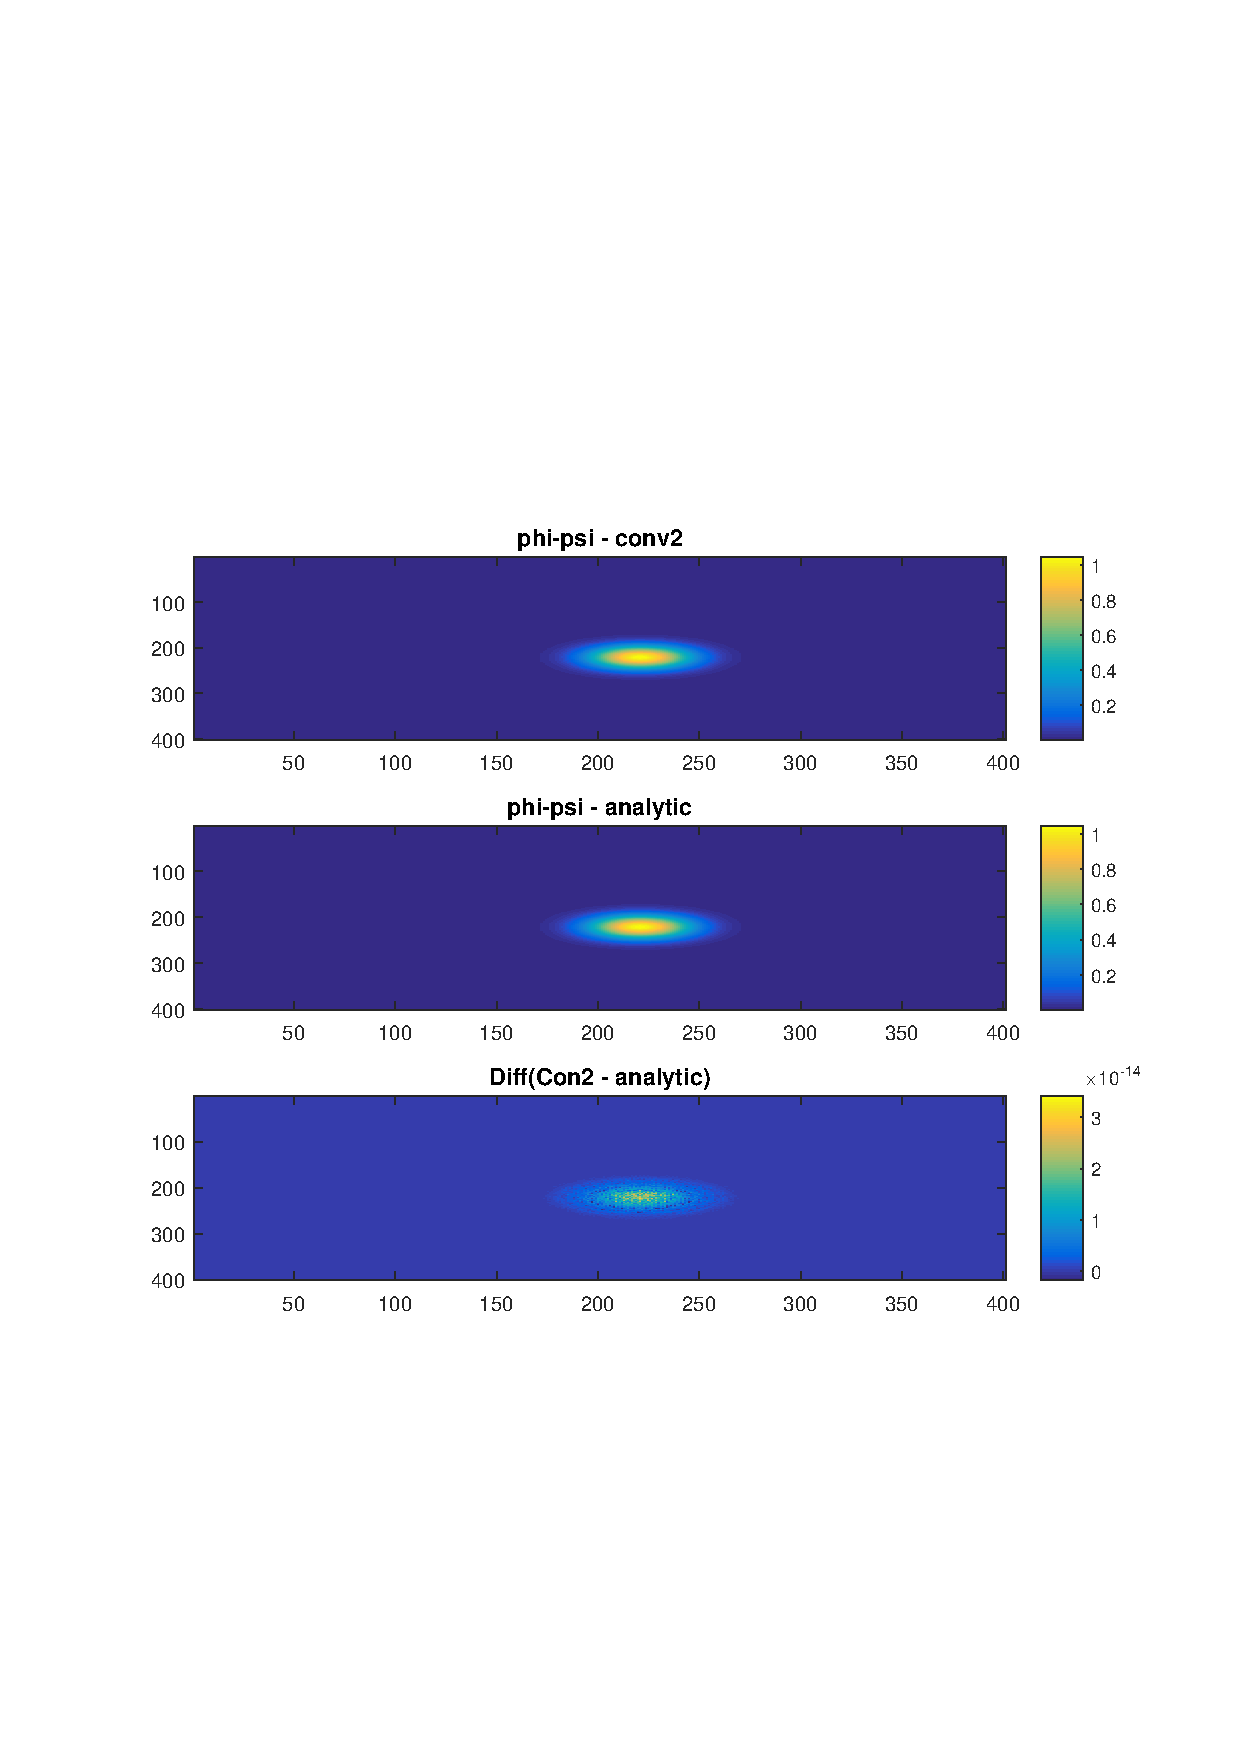
\includegraphics[width=\textwidth]{Convolution2DGaussians_Analytic_Conv2.pdf}
\caption{Residual(analytic, Conv2)}\label{Convolution2DGaussians_Analytic_Conv2.pdf}
\end{figure}



\newpage

\section{Swap the order}
\paragraph{Here is to provide the derivation of swap the order of convolution and inner-product.}


\subsection{Derivation}
Define $\varphi(\boldsymbol{r}) $ and $\psi(\boldsymbol{r}) $ as 2-dimensional Gaussians.
Define $f(\boldsymbol{r}) $ as 2-dimensional random data. The target is prove
$$ \varphi \otimes (\psi \ast f) = (\varphi \ast \psi) \otimes f,   $$
where $\otimes $ is inner product of two Gaussians and $\ast $ is convolution, through derivations and analytic check.

\subsection{Analytical and numerical check}
By running script, \textit{}


\newpage

% Compute Gamma
\section{Compute Gamma}

\paragraph{To analytically compute Gamma Matrix, we define
$\Gamma=\int_{\Omega}\phi(\boldsymbol{r})\phi^{T}(\boldsymbol{r})dr$.
Firstly, we define $\phi(\boldsymbol{r})$ as a vector of Gaussian basis functions.
Each Gaussian basis function is defined as,
$$\phi(\boldsymbol{r}-\boldsymbol{r}\prime)=\exp{\left(-\frac{(\boldsymbol{r}-\boldsymbol{r}\prime)^{T}(\boldsymbol{r}-\boldsymbol{r}\prime)}{\sigma_{\phi}^{2}}\right)}$$}

\paragraph{File (Matlab script): ComputeGamma.m}

\subsection{Parameter List}
\textbf{\textit{Input parameter list:}}\newline
SpaceMin - Edge of surface on the negative side\newline
SpaceMax - Edge of surface on the positive side\newline
NPoints - number of points along each dimension\newline
nx - number of Gaussian basis functions\newline
mu - centres of Gaussians, a 2 times Nx matrix\newline
sigma - variance-covariance matrix of each Gaussian\newline
\textbf{\textit{Output parameter list:}}\newline
gamma - gamma matrix

\subsection{Implementations}
\paragraph{Inner product of two Gaussians\newline}
By definition, Gamma Matrix is defined as,
$$\Gamma = \left(
\begin{array}{ccc}
\varphi_1\otimes\varphi_1&\cdots&\varphi_1\otimes\varphi_{nx}\\
\vdots&\ddots&\vdots\\
\varphi_{nx}\otimes\varphi_1&\cdots&\varphi_{nx}\otimes\varphi_{nx}
\end{array}
\right),$$ each $ \varphi$ is a Gaussian basis function.\par
To compute Gamma Matrix, we compute inner product between each Gaussian basis
function by calling local function, \textit{InnerProductTwo2DGaussians.m}. \newline The inner
product of two Gaussian basis function is defined as below,
$$\varphi_i\otimes\varphi_j=\int_{\mathbb{R}^\mathbb{N}}\varphi_i(\boldsymbol{r})\varphi_j(\boldsymbol{r})\,d\boldsymbol{r},$$
in Equation (D.3) Appendix D.\par
The local function, \textit{InnerProductTwo2DGaussians.m}, analytically computes the
integration of two Gaussian basis functions over the space. This analytic solution
is defined as below,
$$\varphi_i\otimes\varphi_j = \left(\frac{\pi\sigma^2_i\sigma^2_j}{\sigma^2_i+\sigma^2_j}\right)^{\frac{n}{2}}
\times\exp{\left(-\frac{1}{\sigma^2_i+\sigma^2_j}(\mu_i-\mu_j)^T(\mu_i-\mu_j)\right)}, $$
in Equation (D.7) Appendix D.
\subsection{Results}
\begin{figure}[H]
\centering
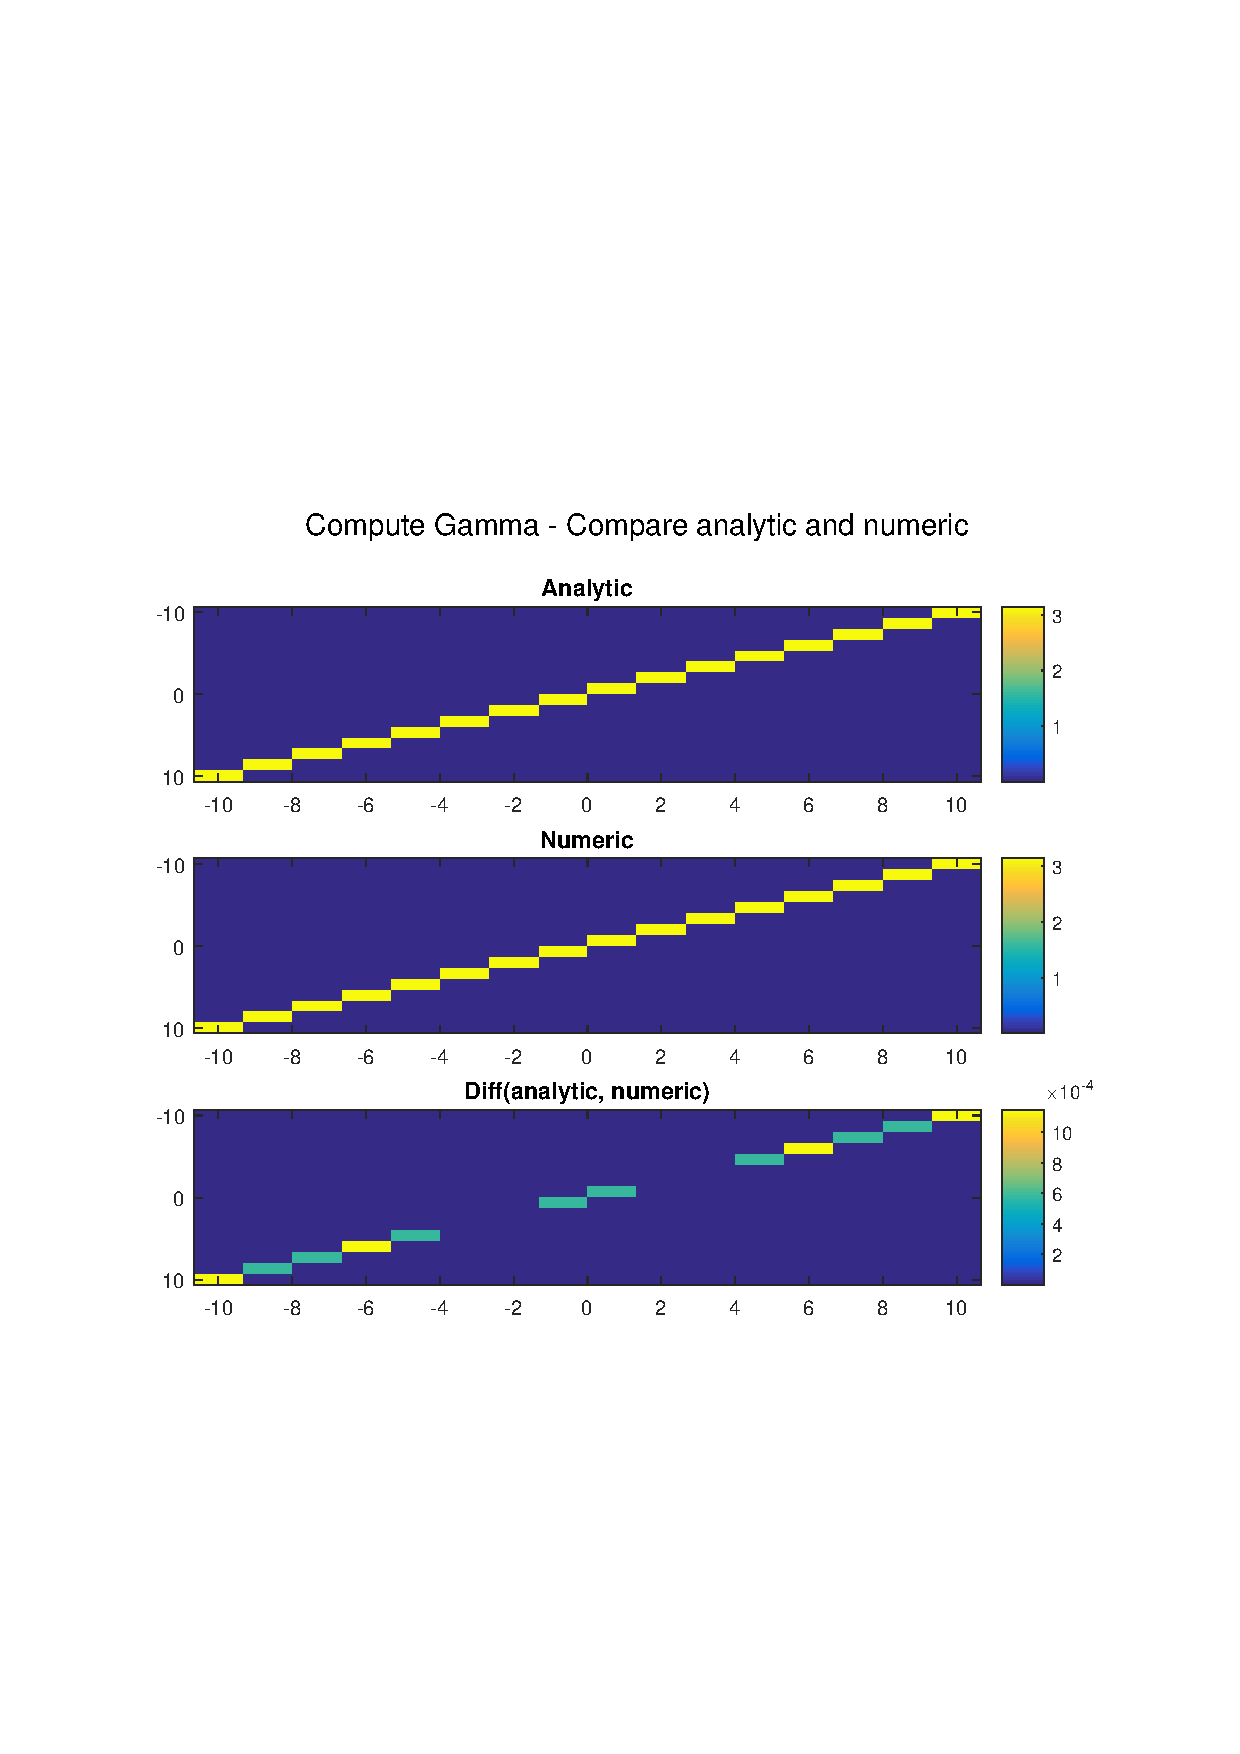
\includegraphics[width=\textwidth]{ComputeGamma_Check_AnalyticNumeric_SpatialRes_501.pdf}
\caption{Compare analytic and numeric results of computing Gamma}
\end{figure}

\newpage



% Compute Psi
\section{Compute Psi}
\paragraph{We will compute Psi Matrix, according to
$$[\Psi(\boldsymbol{r}\prime)]_{:i}= T_s\Gamma^{-1}\int_{\Omega}\phi(\boldsymbol{r})\psi_i(2\boldsymbol{c}_i-\boldsymbol{r}\prime- \boldsymbol{r})\,d\boldsymbol{r},$$
Equation (24). In this section, we
wiil use the Gamma matrix computed from the previous section.}
\paragraph{File (Matlab script): ComputePsi.m}


\subsection{Parameter List}
\textbf{\textit{Input parameters}:}\newline
SpaceMin - Edge of surface on the negative side \newline
SpaceMax - Edge of surface on the positive side \newline
NPoints - number of points along each dimension \newline
nTheta - number of connectivity kernel basis functions \newline
Ts - Time step \newline
nx - number of Gaussian basis functions \newline
mu\_phi - centre of Gaussian basis function for phi \newline
sigma\_phi - sigma of Gaussian basis function for phi \newline
mu\_psi - a vector of centres of Gaussian basis functions of connectivity kernel \newline
vector\_Sigma\_Psi - a vector of sigma of Gaussian basis functions \newline
\textbf{\textit{Output parameters}}:\newline
Psi - Psi matrix



\subsection{Implementations}

\paragraph{Pre-define parameters and centres of field basis functions\newline}
Define the coordinates of discretisation of the cortical surface as varialbe \textit{x}. If the centres of field basis function are left as empy the input parameters (mu\_phi, a
vectore of 2-D coordinates of centres), we define these centres here and spread them
uniformly in the cortical surface. \newline
We calculate the number of rows, \textit{numRow}, and columns, \textit{numCol}, based on the
number of field basis function, \textit{nx}.\newline
We align the centres of field basis functions to either right on the
discretisation points or the middle point of two adjacent discretisation
points, to avode introducing unnecessary dynamics. \newline
So, we have centres, \textit{mu\_phi}, and variance-covariance matrix, \textit{covMat\_phi},
of each field basis functions.\newline
\paragraph{Compute Gamma\newline}
Call function, \textit{ComputeGamma.m}, to compute Gamma matrix, \textit{Gamma} (a \(\textit{nx}\times
\textit{nx}\) matrix).\newline

\paragraph{Compute coefficients of convolution of phi and psi\newline}
A vector of Gaussian coefficients, \textit{psi\_phi\_coefficient} (\(1\times\textit{nTheta}\) vector), is computed based on Equation
(E.4) Appendix E.

\paragraph{Compute convolution of phi and psi\newline}
To compute convolution of psi and phi analytically, we use function \textit{Define2DGaussian\_AnisotropicKernel.m}
to define Gaussian basis and times the coefficients, \textit{psi\_phi\_coefficient}.
The resultant Gaussians are stored in variable \textit{psi\_phi\_basis}

\paragraph{Compute Psi matrix\newline}
Firstly we inverse Gamma matrix as \textit{inv\_Gamma}. Then we times time step, \textit{Ts} (constant), and \textit{inv\_Gamma} to each row of \textit{psi\_phi\_basis}.
The result is Psi matrix and it's stored in variable \textit{Ts\_invGamma\_phi\_psi} and is returned back to the function.

\subsection{Results}
Run script: ComputePsi\_Compare\_AnalyticNumeric.m
\begin{figure}[H]
\centering
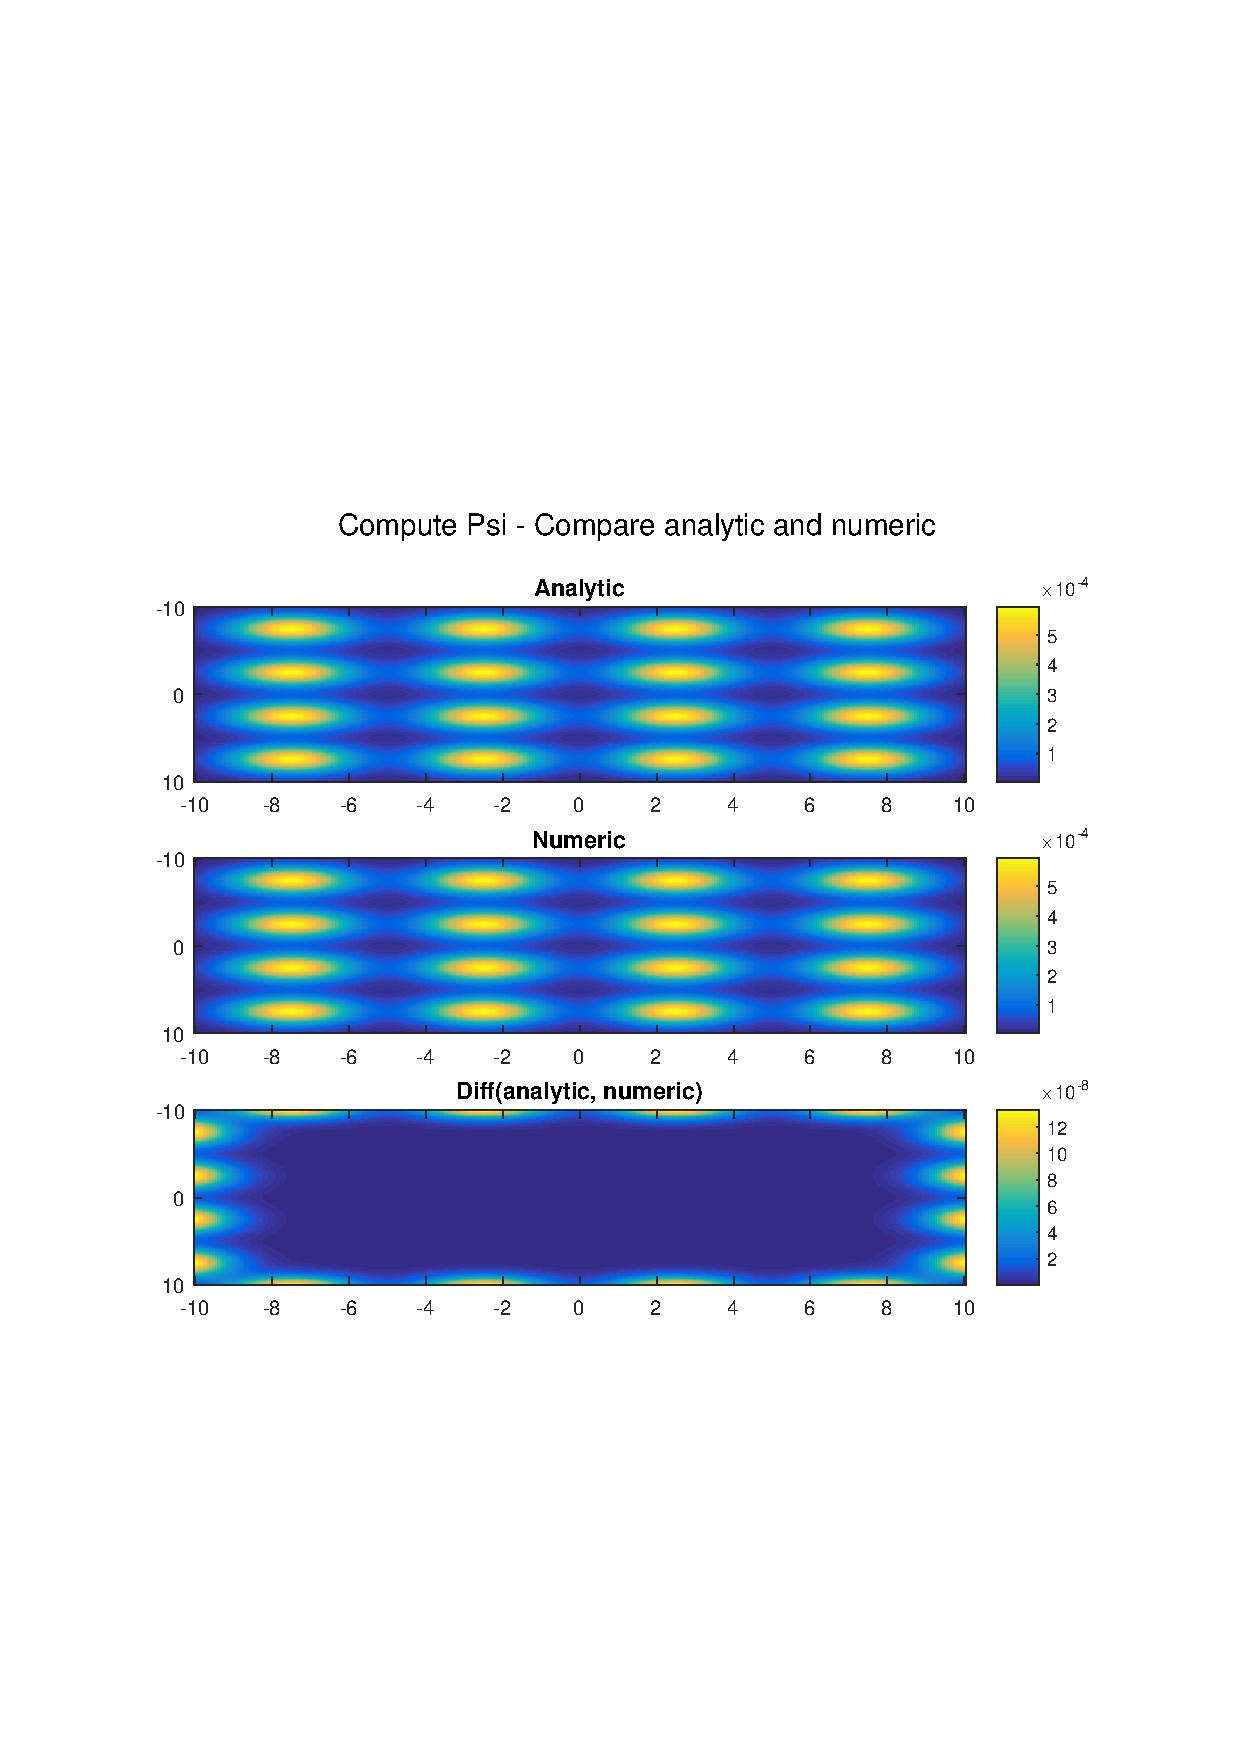
\includegraphics[width=\textwidth]{ComputePsi_Check_AnalyticNumeric_SpatialRes_301.pdf}
\caption{Compare analytic and numeric results of computing Psi}
\end{figure}
\newpage




\section{Compute Reduced Model}

\paragraph{We use analytical solution to compute neural field at time t+1 based on
neural field at time T.\newline
This analytical solution is computed based on equations,
$$\boldsymbol{x}_{t+1}=\int_{\Omega}\Psi(\boldsymbol{r}\prime)f(\phi^{T}(\boldsymbol{r\prime})\boldsymbol{x_t})d\boldsymbol{r}\theta + \xi\boldsymbol{x_t} + \Gamma^{-1}\int_{\Omega}\phi(\boldsymbol{r})e_t(\boldsymbol{r})d\boldsymbol{r},$$
Equation (25) and,
$$v_{t+1}(\boldsymbol{r})\approx\phi^T(\boldsymbol{r})\boldsymbol{x_{t+1}}, $$
Equation (15).\newline
In this implementation, we ignore the error part, $\Gamma^{-1}\int_{\Omega}\phi(\boldsymbol{r})e_t(\boldsymbol{r})$, in Equation (25).\newline
To compute neural fieldt at t+1 with reduced model, we use local functions implemented in the previous sections.
}

\paragraph{File (Matlab script): ReducedModel\_ComputeFieldVtPlus1.m}

\subsection{Parameter List}
\textbf{\textit{Input parameters}:}\newline
Xt - State vector at time t\newline
nx - Number of field basis functions (field decomposition)\newline
sigma\_phi - width of field basis functions (field decomposition)\newline
theta - scale of basis functions of connectivity kernel\newline
nTheta - number of basis functions of connectivity kernel\newline
mu\_psi - widths of basis functions of connectivity kernel\newline
vector\_Sigma\_Psi - a vector of widiths of Gaussian basis functions of
connvectivity kernel (spatial decomposition)\newline
SpaceMin - the negative edge of cortical surface\newline
SpaceMax - the posive edge of cortical surface\newline
NPoints - number of points in each row or column of cortical
surface (spatial resolution)\newline
\textbf{\textit{Output parameters}}:\newline
VtPlus1 - neural field at time t+1\newline
Vt - neural field at time t
(constructed from field basis function and state vector)\newline
XtPlus1 - state vector at time t+1\newline
\subsection{Implementations}

\paragraph{Define spatial parameters of cortical sheet\newline}
Here we define \textit{x} as coordinates of discretisation of the surface and
\textit{stepSize} as distance between two adjacent points in the 2-D surface.
\textit{X} and \textit{Y} are the x-coordinates and y-coordinates of the 2-D surface.

\paragraph{Parameters of reduced model\newline}
ks - $\xi = 1 - T_s\zeta $, where $T_s$ is the time step and $\zeta $ is inverse synaptic time constant. \newline
slope\_sigmoidal - slope of sigmoidal activation function of firing rate function.\newline
v0 - firing threshold of firing rate function.\newline
In this implementation, we set those parameters to the values estimated in the paper.

\paragraph{Create field basis functions - $\phi(\boldsymbol{r}) $\newline}
To create a vector of field basis functions, namely phi, we call a local function,
\textit{CreatePhiBasisFunctions.m}. This function uniformly (centre locations on the cortical sheet)
create Gaussian basis functions, according to variance-covariance matrix, \textit{sigma},
and number of Gaussian basis functions, \textit{nx}.

\paragraph{Compute Psi\newline}
To compute Psi matrix, i.e. $\Psi(\boldsymbol{r\prime}) $ in Equation (25),
we call local function, \textit{ComputePsi.m}. Please see Section Compute Psi
for details.

\paragraph{Firing rate function\newline}
To compute neural field after going through firing rate function, we implement this
part of script according to
$$f(v(\boldsymbol{r\prime}, t)) = \frac{1}{1+\exp(\varsigma(v_0-v(\boldsymbol(r\prime), t)))}. $$\newline
Variable $v_0 $ is the firing threshold $v_0 $ in the equation and \textit{slope\_sigmoidal}
is $\varsigma $ in the firing rate equation.

The input varialbe to firing rate function is $\phi^T(\boldsymbol{r\prime})\boldsymbol{x_{t}} $,
which is the contructed neural field based on state vector and decomposed basis functions.

\paragraph{Integral and state vector at time t+1\newline}
In this part, we first compute the matrix mutiplication of Psi matrix and the matrix from firing rate function,
and this gives us a $nx\times n\theta$ matrix of fields.
By calculting the integral of each field in the previous matrix over space, we are
able to calculate the state vector $x_{t+1} $ according to Equation (25).

\paragraph{Neural field at time t+1\newline}
To constructed the neural field at time t+1, we multiply the state vector computed
in the previous part and field basis functions.

\subsection{Results}
We present the neural field at time t+1 in the Section of Compare Reduced Model and Full Model.

\newpage





\section{Compute Full Model}

\paragraph{We numerically compute neural field at time T+1 based on field at time T.
As opposed to reduced model, full model does not decompose neural field into field basis functions; it directly convolves
the neural field at time t with connectivity kernel, as Equation (12) shown here,
$$v_{t+T_s}(\boldsymbol{r}) = \xi\,v_t(\boldsymbol{r}) + T_s\int_{\Omega}w(\boldsymbol{r}, \boldsymbol{r\prime})f(v_t(\boldsymbol{r\prime}))d\boldsymbol{r\prime} + e_t(\boldsymbol{r}).$$}

\subparagraph{In full model, when we convolve neural field at time T with connectivity kernel,
we have significant errors or residuals on the edges of the field. In order to conquer this,
we apply a boundary condition method to extend the field into 9 tiles and each tile is an identical copy
of the neural field.}

\paragraph{File (Matlab script): CompleteModel\_ComputeFieldVtPlus1.m}

\subsection{Parameters}
\textbf{\textit{Input parameters}:}\newline
Vt - Neural field at time t\newline
theta - scale of basis functions of connectivity kernel\newline
nTheta - number of basis functions of connectivity kernel\newline
mu\_psi - the centre of Gaussian basis function of connectivity kernel\newline
vector\_Sigma\_Psi - a vector of widiths of Gaussian basis functions of
connvectivity kernel (spatial decomposition)\newline
SpaceMin - the negative edge of cortical surface/neural field\newline
SpaceMax - the posive edge of cortical surface/neural field\newline
NPoints - number of points in each row or column of cortical\newline
\textbf{\textit{Output parameters}}:\newline
VtPlus1 - neural field at time t+1\newline

\subsection{Implementations}

\paragraph{Spatial parameters\newline}
Here we define \textit{x} as coordinates of discretisation of the surface and
\textit{stepSize} as distance between two adjacent points in the 2-D surface.
\textit{X} and \textit{Y} are the x-coordinates and y-coordinates of the 2-D surface.


\paragraph{Model parameters\newline}
ks - $\xi = 1 - T_s\zeta $, where $T_s$ is the time step and $\zeta $ is inverse synaptic time constant. \newline
slope\_sigmoidal - slope of sigmoidal activation function of firing rate function.\newline
v0 - firing threshold of firing rate function.\newline
In this implementation, we set those parameters to the values estimated in the paper.

\paragraph{Boundary condition\newline}
In this implementation, we programed two boundary conditions, 9 tiles and symmetry condition.
In both boundary conditions, we extend the current neural field into a $3\times3 $ field.
The extended field is called \textit{extendedField} in the implementation.
In 9-tile condition, each tile is the identical copy of the original field.
In symmetry condition, each edge of the orignal field becomes a mirror and
each tile is the mirrored field of the original field.

\paragraph{Convolution\newline}
In this part, we convolve the extended field with the connectivity kernel
that we define based on input parameters. After this convolution, we crop the
centre or the middle field of the extended field as the convolved field.\par

In the script, we use variable \textit{w} as the connectivity kernel and
\textit{extendedField} as the solution of boundary condition.
The convolution implements
$ T_s\int_{\Omega}w(\boldsymbol{r}, \boldsymbol{r\prime})f(v_t(\boldsymbol{r\prime}))d\boldsymbol{r\prime}$
in the Equation (12).

\paragraph{Neural field at time t+1\newline}
Finally, given the convolution result from previous part and Equation (12),
we are able to directly calculate the neural field at t+1.

\subsection{Results}
We present the neural field at time t+1 in the Section of Compare Reduced Model and Full Model.
\newpage


\section{Compare Reduced Model and Full Model}
\paragraph{Compare neural fields at time T+1 computed by reduced model and full model.}

\paragraph{Script name: Compare\_CompleteModel\_ReducedModel.m}

\subsection{Parameters}

tau - synaptic time constant.\newline
Ts - time step.\newline
SpaceMin - the negative edge of cortical surface.\newline
SpaceMax - the posive edge of cortical surface.\newline
NPoints - number of points in each row or column of spatially discretised cortical surface.\newline
nx - number of Gaussian basis function of field decomposition.\newline
sigma\_phi - Variance-covariance matrix of Gaussian basis function of field decomposition.\newline
theta - Scales of Gaussian basis functions of connectivity kernel.\newline
nTheta - Number of connectivity kernel basis functions.\newline
mu\_psi - Centres of basis functions of connectivity kernel.\newline
vector\_Sigma\_Psi - a vector variance and covariance of Gaussian basis functions of connectivity kernel.\newline
Xt - state vector at time t.
To simulate neural field model, we generate a vector of random numbers each time.

\subsection{Implementation}
In fact, we want to test two types of connectivity kernels, Mexican hat and Gabor kernel.
In order to conveniently switch between different types of connectivity kernels,
we parameterised connectivity kernels into centres of basis functions, \textit{mu\_psi},
and a vector of variance-covariane matrices, \textit{vector\_Sigma\_Psi}.
Therefore, by changing the number of basis functions and variance-covariance matrices,
we will have different connectivity kernels.


\paragraph{Mexican hat kernel\newline}
To test our implementation of neural field model, we compute neural field at time
t+1 from reduced model and full model based on the same state vector at time t.
We compare the residual or errors by subtracting neural field of full model
from that of reduced model. By visualising generated neural field at time t,
neural field generated from reduced model and full model and their residual,
we are able to qualitatively assess our implementation.\par
In order to quantitatively assess the our implementation, we calculate the sum of squared
residual matrix as a measure and compare this measure
across multiple spatial resolutions and connectivity kernels.


\paragraph{Gabor kernel\newline}
By changing number of basis functions and variance-covariance matrices of
connectivity kernel, we are able to visualise and quantitatively assess the model
using the Gabor kernel as connectivity kernel. The assessment is the same way as the above.
The results are shown in the next section.


\subsection{Results}

\begin{figure}[H]
\centering
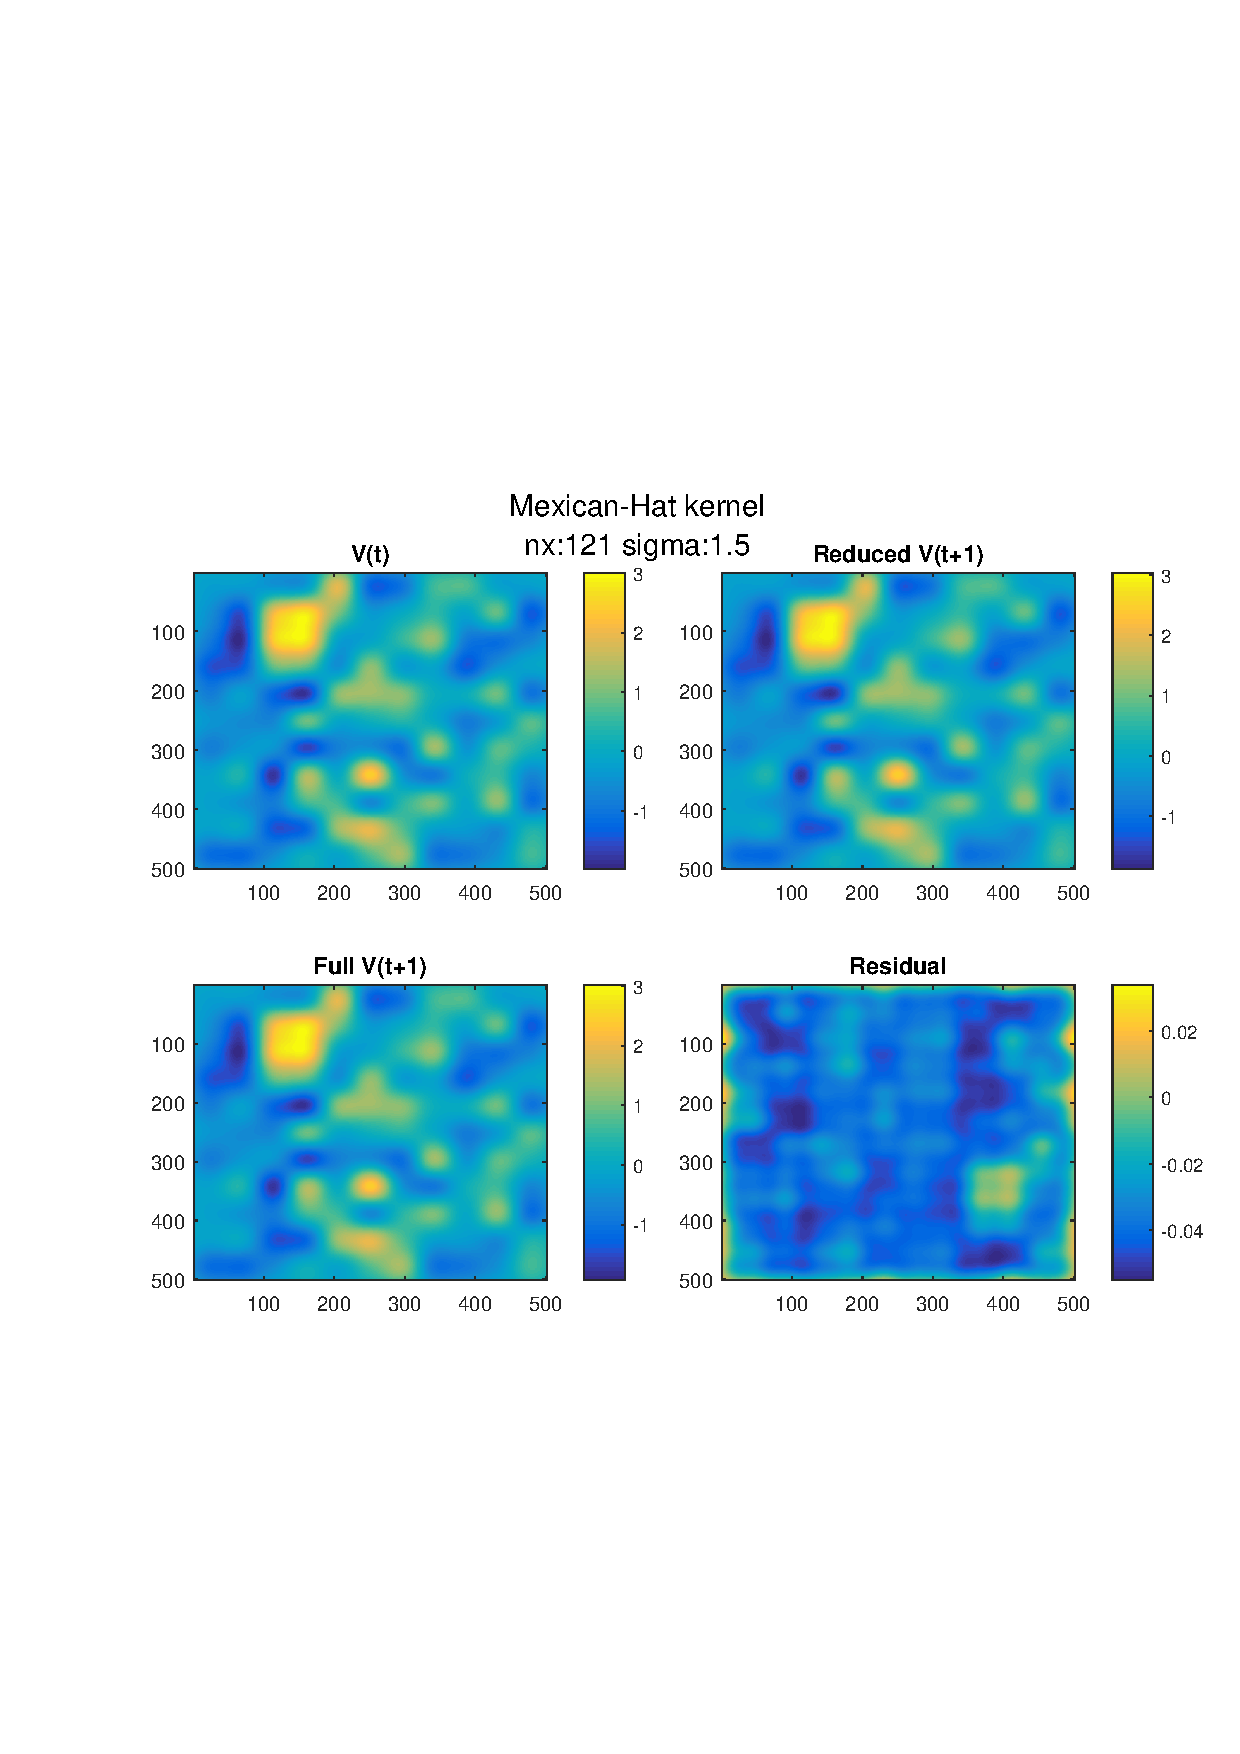
\includegraphics[width=\textwidth]{modelComparison_MexHat_nx_121_sigma_1_5_nPoints_501_vTPlus1.pdf}
\caption{Connectivity kernel, Mexican Hat}
\end{figure}

\begin{figure}[H]
\centering
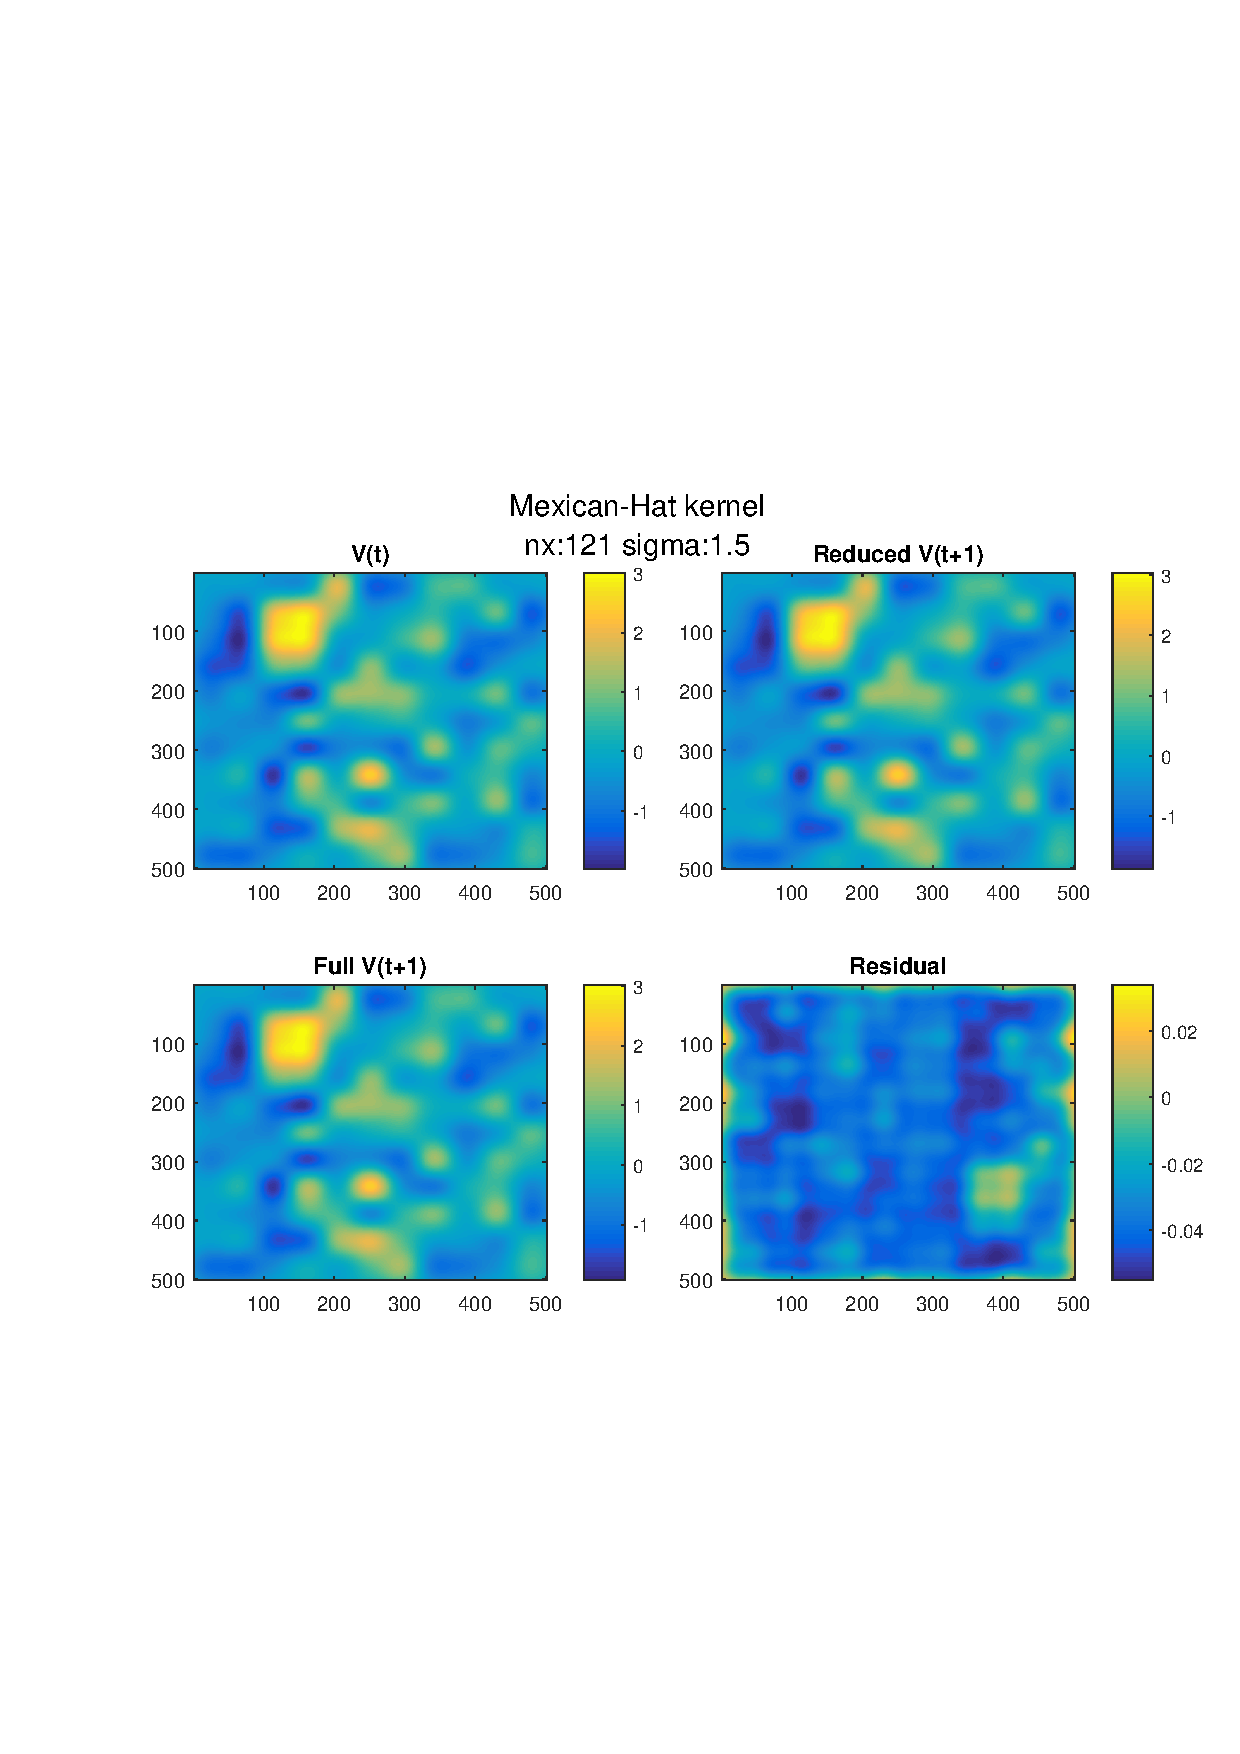
\includegraphics[width=\textwidth]{modelComparison_MexHat_nx_121_sigma_1_5_nPoints_501_vTPlus1.pdf}
\caption{Connectivity kernel, Mexican Hat}
\end{figure}
\end{document}

\subsection{Discussion}
